\documentclass[aspectratio=169]{beamer}

\usepackage{listings}
\usepackage{pdfpcnotes}

% \usepackage{qrcode} doesn't work easily with white-on-black

\usepackage{url}
\usepackage[utf8]{inputenc}

\title{Asynchronous Rust in Embedded Systems}
\author{Christian Amsüss \url{<christian@amsuess.com>}\\\texttt{@chrysn}}
\date{2024-02-29\\Vienna, Rust meetup}

\setbeamertemplate{footline}[frame number]

% source code inclusion
\usepackage{navigator}
\embeddedfile[Build using this Makefile]{makefile}{./Makefile}
\embeddedfile[LaTeX source code]{sourcecode}{./slides.tex}

\usecolortheme{albatross} % easiest base for white-on-black
\setbeamercolor{titlelike}{bg=black,fg=white}
\setbeamercolor{normal text}{bg=black,fg=white}

\begin{document}

\frame{\titlepage}

\begin{frame}{Embedded systems}\Large
  \begin{itemize}
    \item single chip
    \item $\approx 100$ KiB ROM, $< 100$ KiB RAM
    \item Serial, I2C, analog pins, simple networking ($< 1$Kbps)
  \end{itemize}
  \pnote{
    Arduino up to ESP32
\\
    WiFi only on big chips b/c complex and power hungry
\\
    Automation, sensors}
\end{frame}

\begin{frame}{Execution model: bare metal}\Large
  \center
  \vspace{-1em}
  \includegraphics[height=\textheight]{baremetal.pdf}


\pnote{
  single entry point, code runs at full privileges.
  \\
  some default stack.
  \\
  (memory: stack, statics, ?heap)
}
\end{frame}

\begin{frame}[fragile]{Execution model: bare metal}\Large
\framesubtitle{No parallelism}
  \begin{verbatim}
  loop:
      if button pressed:
          increase counter
      if socket.is_pending():
        connection = socket.accept()
        connection.recv(...)
        connection.send(...)
        connection.close()
  \end{verbatim}
\end{frame}

\begin{frame}[fragile]{Execution model: bare metal}\Large
\framesubtitle{Interrupts}
  \begin{verbatim}
  on button_pressed():
      increase counter

  on network activity():
      ... (see next slide)
  \end{verbatim}
\pnote{
  interrupts: configured -- at external event, run code.
  \\
  own stack or shared stack
  \\
  often DMA (eg. audio readout).
}
\end{frame}

\begin{frame}[fragile]{Execution model: bare metal}
\framesubtitle{Hand rolled parallelism}
  \begin{verbatim}
  connection = None
  loop:
      if button pressed:
          increase counter
      if let event = socket.take_pending():
          if connection:
              match event:
                  new connection: reject
                  new data: receive and process
                  ready to send: send(); close(); connection = None
          else:
              match event:
                  new connection: connection = Some(accept())
                  _: reject
  \end{verbatim}
\pnote{
    error prone manual work
    \\
    state machine building
    \\
    interrupts wind up similar if complex
  \\
  \\
  Racking up stack space at the top
}
\end{frame}

\begin{frame}{Execution model: threads}\Large
  \center
  \vspace{-1em}
  \includegraphics[height=\textheight]{threads.pdf}
\pnote{
  "at any time"1: store CPU state ~onto stack,\\
  reconfigure stack. \\
  \\
  restore CPU state from other stack \\
  (incl program counter), continue there \\
  \\
  1: voluntarily from running task, or \\
  by configured interrupt (including timer)
}
\end{frame}

\begin{frame}[fragile]{Execution model: threads}
\framesubtitle{Idiomatic parallelism}
  \begin{verbatim}
  button_main():
      if button pressed:
          increase counter

  network_main():
      loop:
        connection = socket.accept()
        connection.recv(...)
        connection.send(...)
        connection.close()
  \end{verbatim}
  \pnote{
code style: logical per task
\\
downsides:
\\
* task switching (not too bad any more now that there's HW support)
\\
* much RAM use for each task
\\
 -- hard to predict (tools exist but meh), often need to measure, or use more
  \\
 -- different tasks that need to do larger crypto ops would each need stack
  \\
* platform dependent primitives
\\
}
\end{frame}

\begin{frame}{Communication between threads}
\framesubtitle{\ldots and interrupts}\Huge
  \texttt{T: Send}
\pnote{
  Threads?
  \\
  (go back) Criterion: Preemption possible
  \\
  Same for interrupts
  }
\end{frame}

\begin{frame}{Execution model: async}\Large
  \center
  \vspace{-1em}
  \includegraphics[height=\textheight]{tasks.pdf}
\end{frame}

\begin{frame}[fragile]{Execution model: async}
\framesubtitle{Idiomatic parallelism with explicit yielding}
  \begin{verbatim}
  async button_main():
      if button pressed.await:
          increase counter

  async network_main():
      loop:
        connection = socket.accept().await
        connection.recv(...).await
        connection.send(...).await
        connection.close()
  \end{verbatim}
  \pnote{
map back to enums on prev page\\
\\
* (still some dependency on platform primitives,\\
  but can avoid at cost of slightly less efficient spawning)
\\
* one blocks, all block (so don't block)
\\
\\
main argument: convenience without task complexity \\
works well, has tools
}
\end{frame}

\begin{frame}[fragile]{Async: Tools and further reading}\Large
\framesubtitle{Get started with it!}
  \begin{itemize}
    \item \texttt{core}
    \item \texttt{embedded-hal-async}
    \item \texttt{embedded-nal-async}
    \item \texttt{embassy}
    \item RIOT-OS
  \end{itemize}

  \bigskip

  \begin{itemize}
    \item \href{https://onevariable.com/blog/interrupts-is-threads/}{Interrupts Is Threads (James Munns)}
    \item \href{https://ferrous-systems.com/blog/embedded-concurrency-patterns/}{Embedded Concurrency Patterns (Ferrous Systems)}
  \end{itemize}
  \pnote{
... can be combined with multiple executors\\
    (eg. for different priorities) \\
... multi-core work stealing possible but requires Send,\\
    and we often don't have multi cores (or use them differently) \\
  }
\end{frame}

\begin{frame}{}\large
    Thanks for having me here

    \vspace{1cm}

    Slides and more links on \url{https://github.com/RustVienna/meetup-history/tree/master/2024-02/embedded-async/}

    \bigskip
    \center \includegraphics[width=3.2cm]{qr.eps}

    \bigskip

    \hfill Christian Amsüss \url{<christian@amsuess.com>}, \texttt{@chrysn}
\end{frame}\Large

\end{document}
